\documentclass{beamer}
%
% Choose how your presentation looks.
%
% For more themes, color themes and font themes, see:
% http://deic.uab.es/~iblanes/beamer_gallery/index_by_theme.html
%
\mode<presentation>
{
  \usetheme{default}      % or try Darmstadt, Madrid, Warsaw, ...
  \usecolortheme{default} % or try albatross, beaver, crane, ...
  \usefonttheme{default}  % or try serif, structurebold, ...
  \setbeamertemplate{navigation symbols}{}
  \setbeamertemplate{caption}[numbered]
} 

\usepackage[portuguese]{babel}
\usepackage[utf8x]{inputenc}

\title[Análise Complexidade Artigo]{Machine Learning Applications}
\author{Otaviano da Cruz Neto}
\institute{Universidade Federal Fluminense - ICEX VR}
\date{\today}

\begin{document}

\begin{frame}
  \titlepage
\end{frame}

% Uncomment these lines for an automatically generated outline.
%\begin{frame}{Outline}
%  \tableofcontents
%\end{frame}

\begin{frame}{Recognize Handwritten Digits}

\begin{figure}
	\centering
	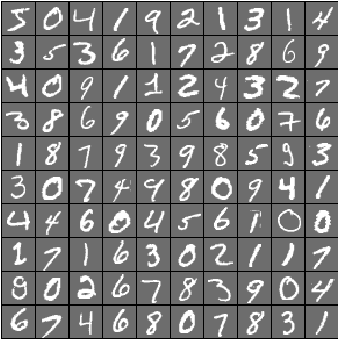
\includegraphics[width=0.7\textwidth]{digits.png}
\end{figure}
	
	
\end{frame}

\begin{frame}{Introdução}

\begin{itemize}
	
	\item \textbf{Individual Data ($X^{(i)}$,$Y^{(i)}$)}
	\begin{equation}
	X^{(i)} = \left[  x_1, x_2, \cdots, x_m \right] 
	\end{equation}
	\begin{equation}
	Y^{(i)} = y^{(i)}  
	\end{equation}
	\item \textbf{Data Sample(X e Y)}
	\begin{equation}
	X = \left[ \begin{array}{rrccccrr}
	1 &&& x_1^{(1)} && \cdots && x_m^{(1)} \\ 
	1 &&& x_1^{(2)} && \cdots && x_m^{(2)} \\
	\vdots &&& \vdots && \cdots && \vdots \\
	1 &&& x_1^{(N)} && \cdots && x_m^{(N)} 
	
	\end{array} \right]
	\end{equation}
\end{itemize}
\end{frame}

\begin{frame}{Introduction} 
\begin{equation}
Y = \left[
\begin{array}{rrcrr}
y^{(1)}\\
y^{(2)}\\
\vdots \\
y^{(N)}
\end{array}
\right]
\end{equation}
\begin{itemize}
\item \textbf{Weight Vector}
\begin{equation}
W = \left[w_0, w_1, w_2, \cdots, w_m\right]
\end{equation}
\item \textbf{Linear Hypotheses }
\begin{equation}
h(w) = X W^T
\end{equation}

\end{itemize}
\end{frame}

\begin{frame}{Logistic Regression}
\begin{itemize}
	\item \textbf{Classification}
	
	The classification is a regression problem which associates a discrete values for each data. In this case we will analyze for binary classification. 
	\item \textbf{Logistic Regression}
	The logistic regression uses probability of each data sample be classified by two discrete values. The logistic regression hypotheses is described by Sigmoid Function,    
	
	\begin{equation}
	h_w(X^{(i)}) = \frac{1}{1 + e^{-X^{(i)}W^T}}
	\end{equation}
	

\end{itemize}
\end{frame}

\begin{frame}{Logistic Regression}
\begin{itemize}
\item \textbf{Sigmoid Function}

\begin{figure}
	\centering 
	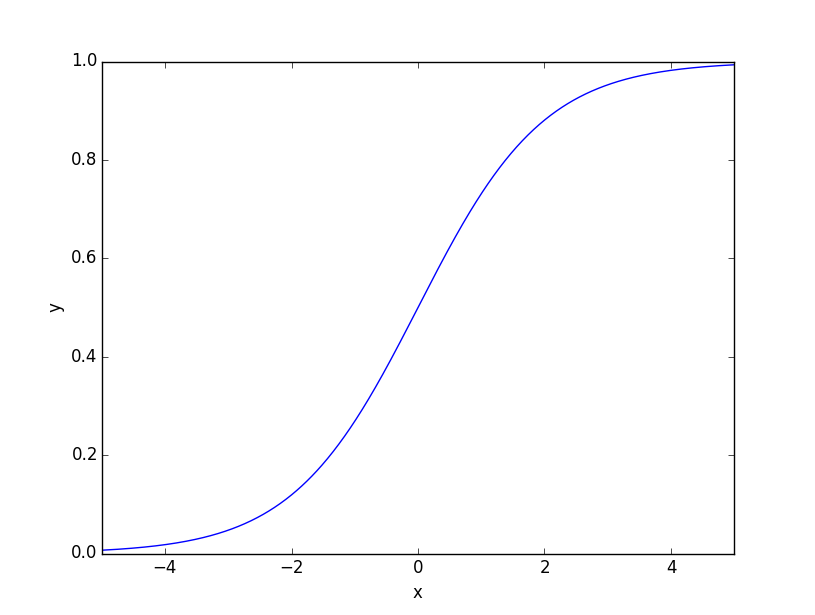
\includegraphics[width=0.6\textwidth]{sigmoid.png}
\end{figure}
\end{itemize}
\end{frame}

\begin{frame}{Logistic Regression}
\begin{itemize}
\item \textbf{Decent Gradient }

To use this technique is necessary calculate the derivative of Sigmoid Function,
\begin{equation}
\begin{split}
\frac{d}{dW}h_W (X^{(i)}) = \frac{1}{1 + e^{-X^{(i)}W^T}}\left( 1 - \frac{1}{1 + e^{X^{(i)}W^T}} \right) \\= h_W(X^{(i)})(1 - h_W(X^{(i)}))
\end{split}
\end{equation}
\end{itemize}
\end{frame}


\begin{frame}{Logistic Regression}

For each classification is valid,

\begin{equation*}
P(Y^{(i)} = 1 | X^{(i)},W) =  h_W (X^{(i)})
\end{equation*}
\begin{equation*}
P(Y^{(i)} = 0 | X^{(i)},W) = 1 - h_W (X^{(i)})
\end{equation*}
This conditional probability have a functional expression :
\begin{equation}
p(Y^{(i)}|X^{(i)},W) = (h_W(X^{(i)}))^{Y^{(i)}}(1 - h_W(X^{(i)}))^{1-Y^{(i)}}
\end{equation}
\end{frame}

\begin{frame}{Logistic Regression}

The probability for N numbers of IID (Independent and Identical Distribution) sample is defined by, 
\begin{equation}
L(W) = \prod_{i = 1}^N (h_W(X^{(i)}))^{Y^{(i)}}(1 - h_W(X^{(i)}))^{1-Y^{(i)}}
\end{equation}
Is necessary maximize as log(L(W)):
\begin{equation}
\sum_{i=1}^N Y^{(i)} \log h_W(X^{(i)}) + (1 - Y^{(i)}) \log( 1 - h_W(X^{(i)}))
\end{equation}
Implying in the algorithm,
\begin{equation}
W_{t+1} = W_t + \alpha (Y^{(i)} - h_W(X^{(i)}))X^{(i)}
\end{equation}
\end{frame}

\begin{frame}{Example}
\begin{figure}
\centering
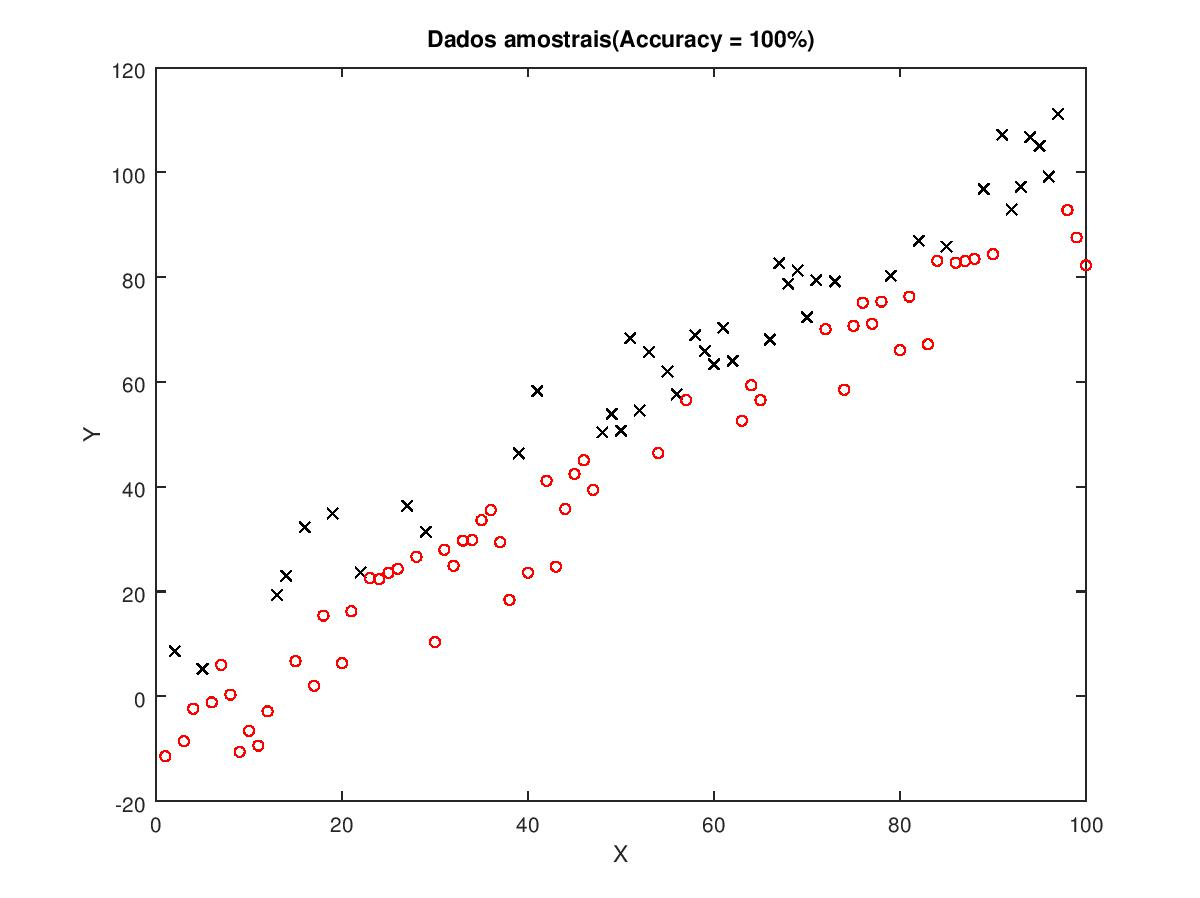
\includegraphics[width= 0.8\textwidth]{Amostra.jpg}
\caption{Binary Data Sample. }
\end{figure}
\end{frame}

\begin{frame}{Example}
\begin{figure}
\centering
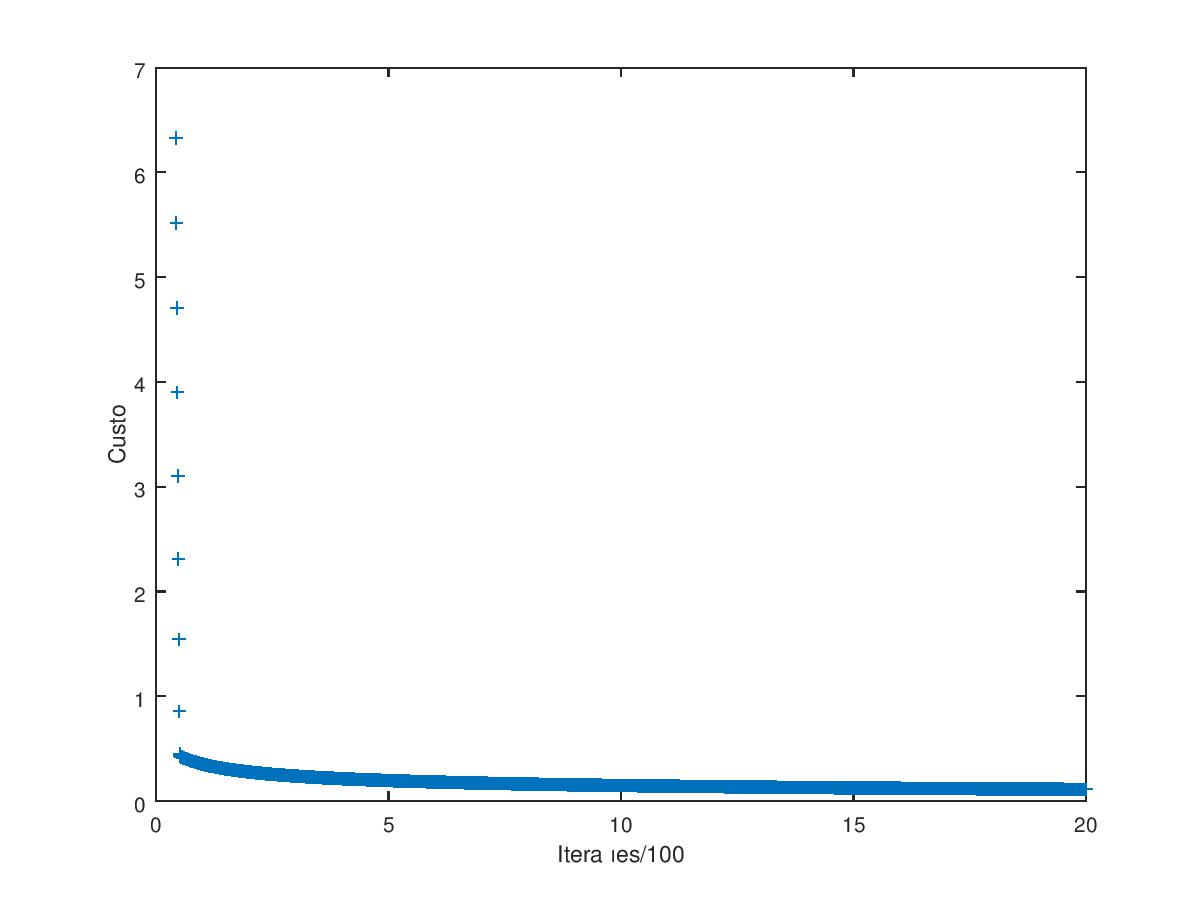
\includegraphics[width=0.8\textwidth]{Custo.jpg}
\caption{Cost function for number of iteration.}  
\end{figure}
\end{frame}

\begin{frame}{Example}
\begin{figure}
\centering
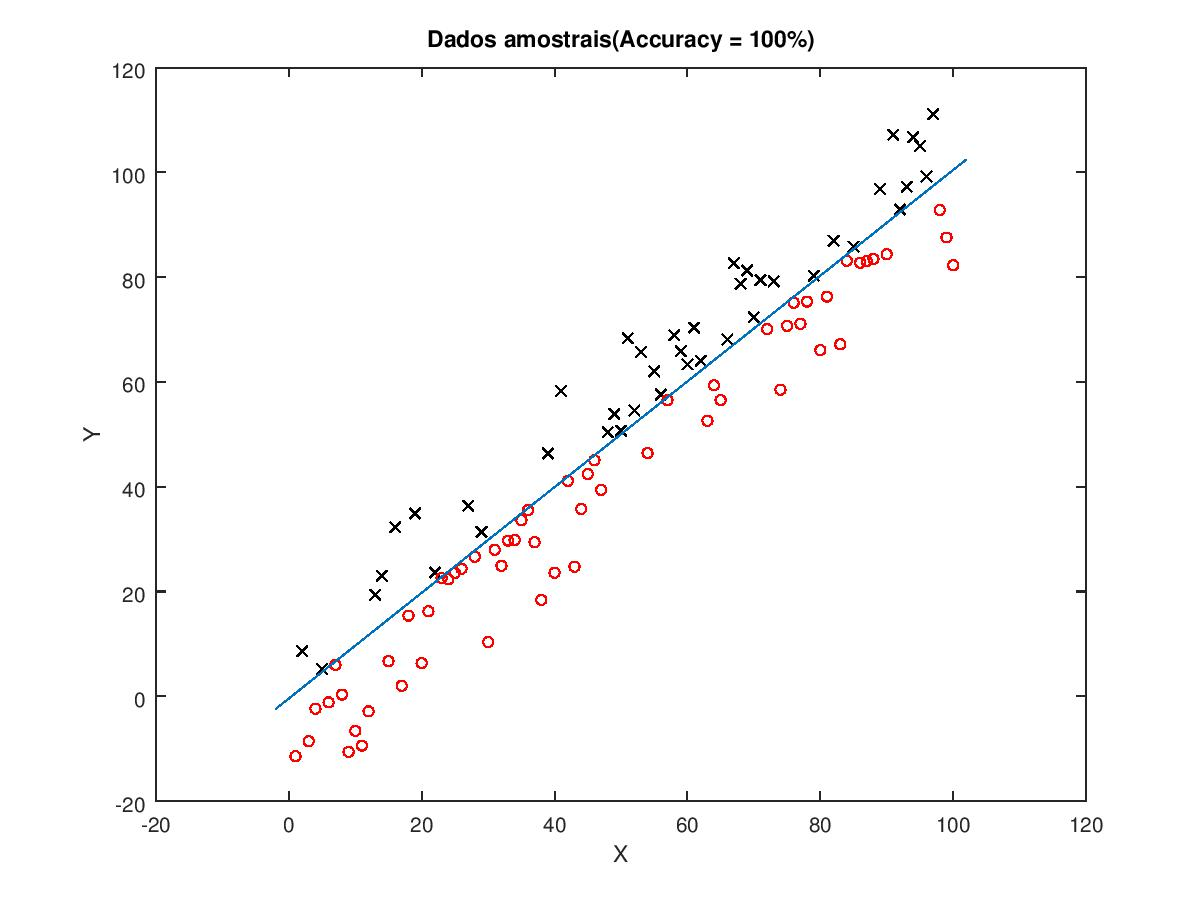
\includegraphics[width=0.8\textwidth]{General.jpg}
\caption{Binary Data Sample and Decision Boundary.}
\end{figure}
\end{frame}


\begin{frame}{Overfitting}

Overfitting is a term used for describe a statistical model whose efficiency is very good in sample but out of sample is worse due to present a random factor and  measurement errors. To fix this is necessary to apply the Regularization whose purpose is to limit the sum of weights. In the Logistic Regression is applied in Decent Gradient as,$\lambda$ is regularization parameter,

\begin{equation}
w^0_{t+1} = w^0_t + \alpha x_0 ' (Y - H_{w_0}(x_0))
\end{equation}

\begin{equation}
w^{(i)}_{t+1} = w^{(i)}_{t} (1 - \alpha\frac{\lambda}{N}) + \frac{\alpha}{N} X^{(i)}' (Y - H_w(X^{(i)}))
\end{equation}

\end{frame}

\begin{frame}{Multi-classification}
\begin{itemize}
\item \textbf{One Vs All} : 

\begin{figure}
\centering
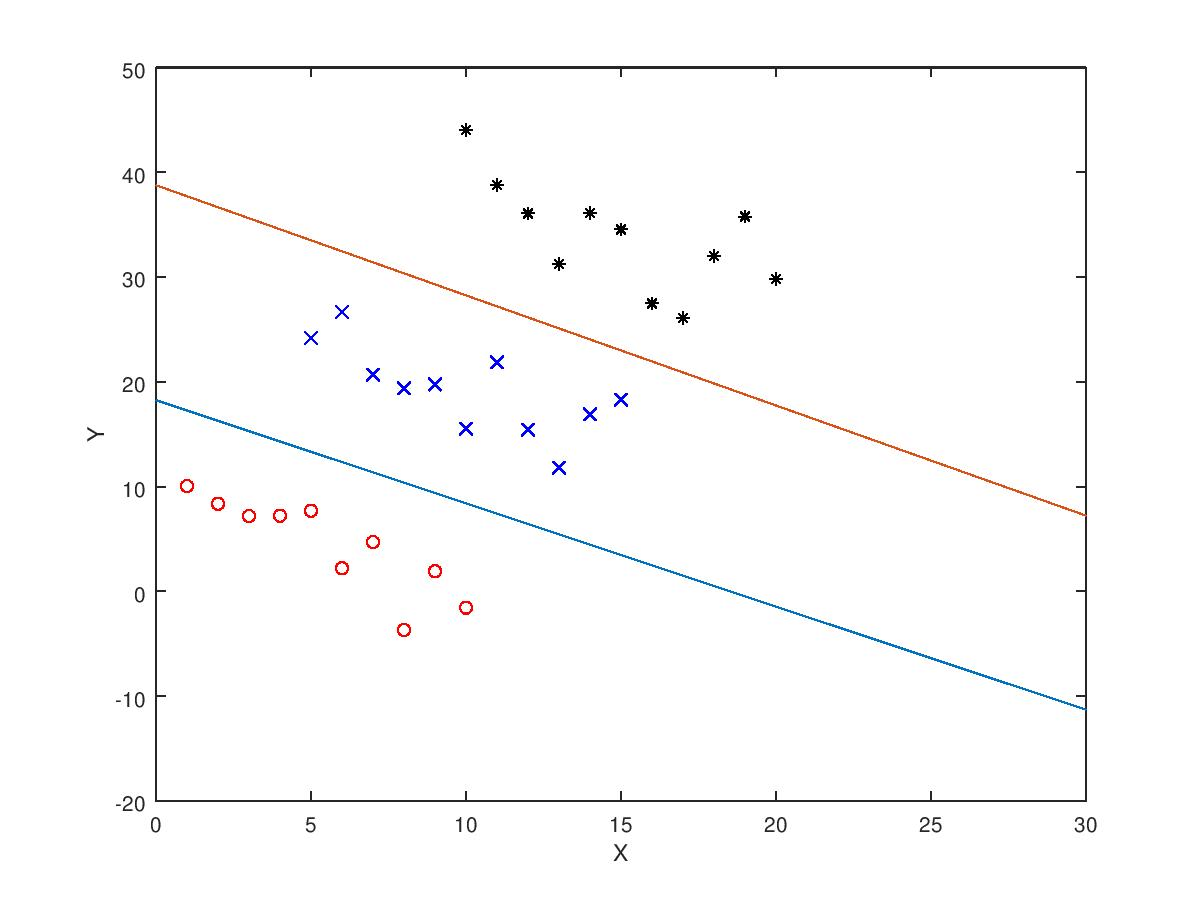
\includegraphics[width=0.8\textwidth]{Amostra_Multi_Class.jpg}
\caption{Data Sample and Boundary Decision.}

\end{figure}	
\end{itemize}
	

\end{frame}

% =====================Complexidade de Imagens================================ %

\begin{frame}{Computerized Measures of Visual Complexity}

\begin{figure}
	\centering
	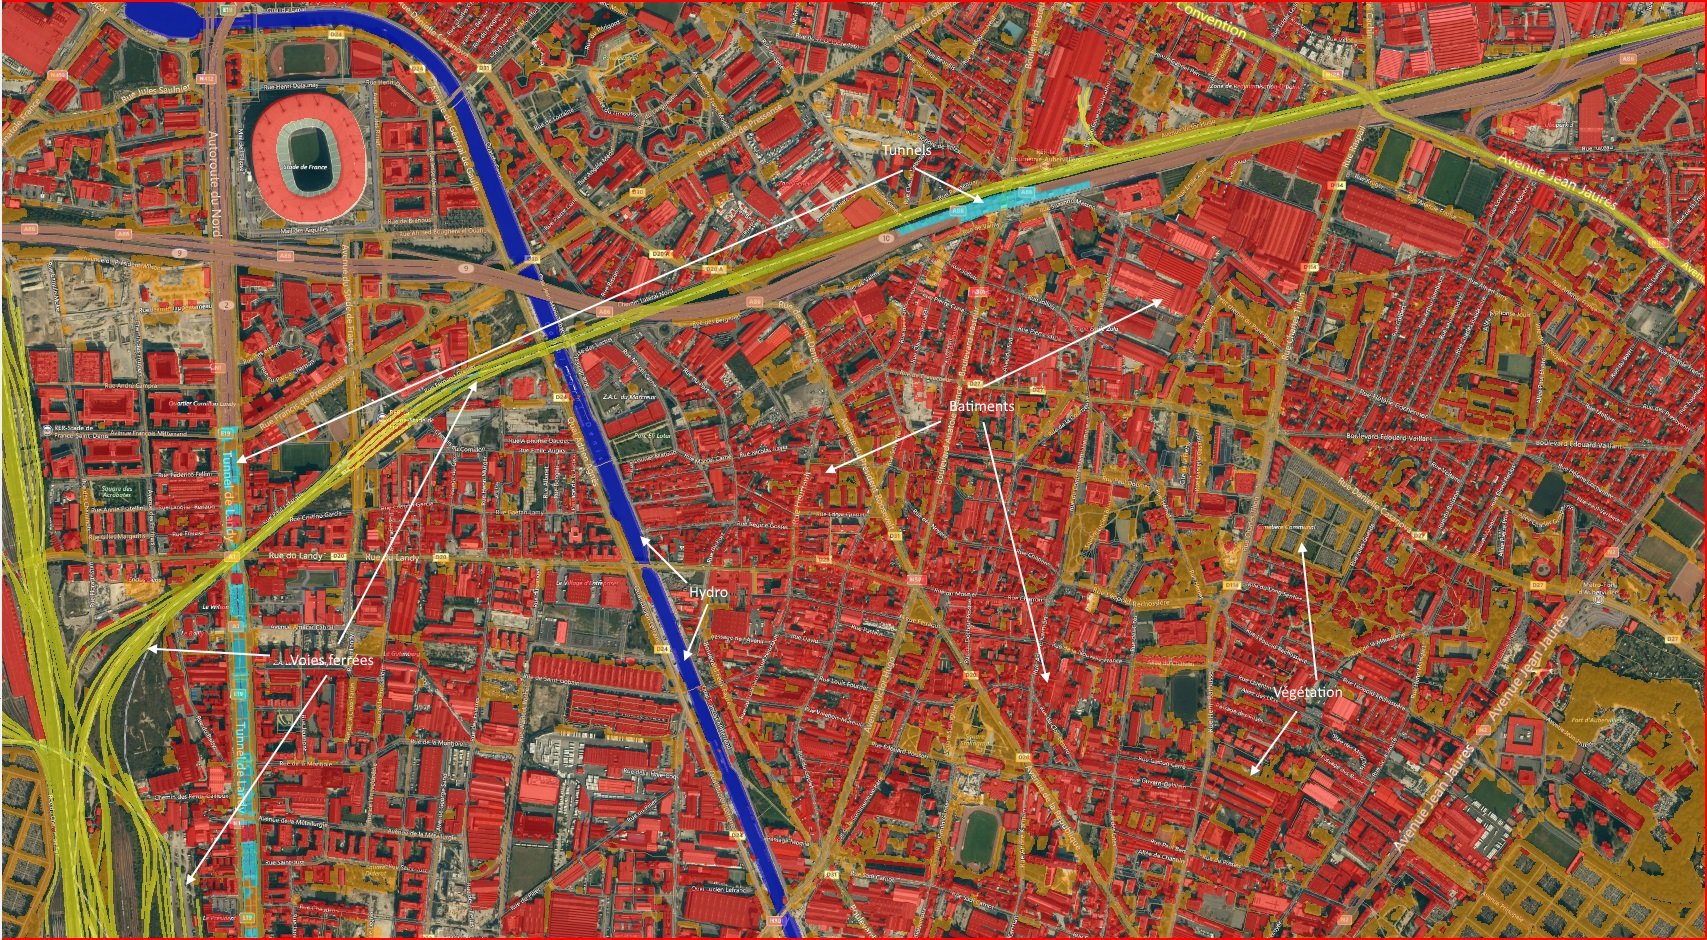
\includegraphics[width=0.7\textwidth]{Ex_Clutter.jpg}
\end{figure}

\end{frame}

 \begin{frame}{Computerized Measures of Visual Complexity}
    \textbf{Types of Images} : 
    \begin{itemize}
        \item Abstract Artistic, Abstract Non-Artistic, Representational Artistic, Representational Non-Artistic, pictures of some natural situations and human-made objects.
    \end{itemize}
    \textbf{Separation}:
    \begin{itemize}
        \item \textbf{Experiment} : Uses some tools and compression formats of images(JPEG and Fractal Compression, edge filter, HSV channel) to extract important information about image complexity, based on human experience and some information like average complexity and medium standard deviation associated.
    \end{itemize}
    
\end{frame}

\begin{frame}{Computerized Measures of Visual Complexity}
    \begin{itemize}
        \item \textbf{Machine Learning} : Utilize machine learning techniques (Artificial Neural Network) and data (average, standard deviation) to recognize some patterns at learning image complexity with efficiency. 
    \end{itemize}
\end{frame}
\begin{frame}{Features}
	The article utilize only 2 features (Compression Method and Edge Dispersion [Canny, Sobel]) because at high correlation.
    \begin{itemize}
        \item \textbf{Compression Method} : The compression method is a indicator of image complexity because of algorithm routine, that routines identify recurring pixels to reduce image file size. We use this to observe how predictable is the image.
        \item \textbf{ Edge Dispersion } : The Image`s Edge Dispersion is a good contribution for research area because of the high  correlation.
    \end{itemize}
\end{frame}


\begin{frame}{Statistical Analyses}

The correlation is defined by Pearson Correlation Coefficient(PCC).

\begin{itemize}
	\item \textbf{PCC}: relates two variables to calculate the linear correlation between them.
\end{itemize}

\begin{equation}
PCC = \frac{\sum_{j = 1}^{N} (f(x_j) - \bar{f(x)})(y_j - \bar{y})}{\sqrt{\sum_{j =1}^{N} (f(x_j) - \bar{f(x)})^2 \sum_{j = 1}^{N} (y_j - \bar{y})^2 }}
\end{equation}
\end{frame}

\begin{frame}{Algorithm}
    Utilizes how is the dependency between Edge Filters (Canny, Sobel), average, HSV Channels, Standard Deviation.

    \begin{figure}
        \centering
        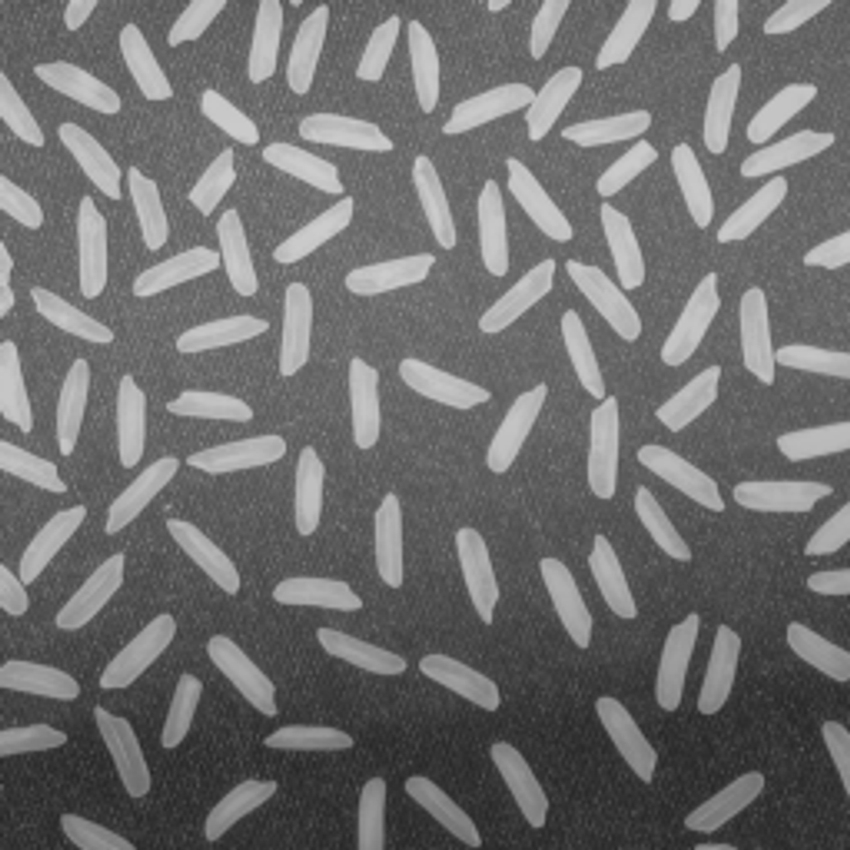
\includegraphics[width=0.5\textwidth]{rice.jpg}
        \caption{Image without edge filter.}
        \label{Bordas}
    \end{figure}
\end{frame}

\begin{frame}{Results}
    \begin{figure}
        \centering
        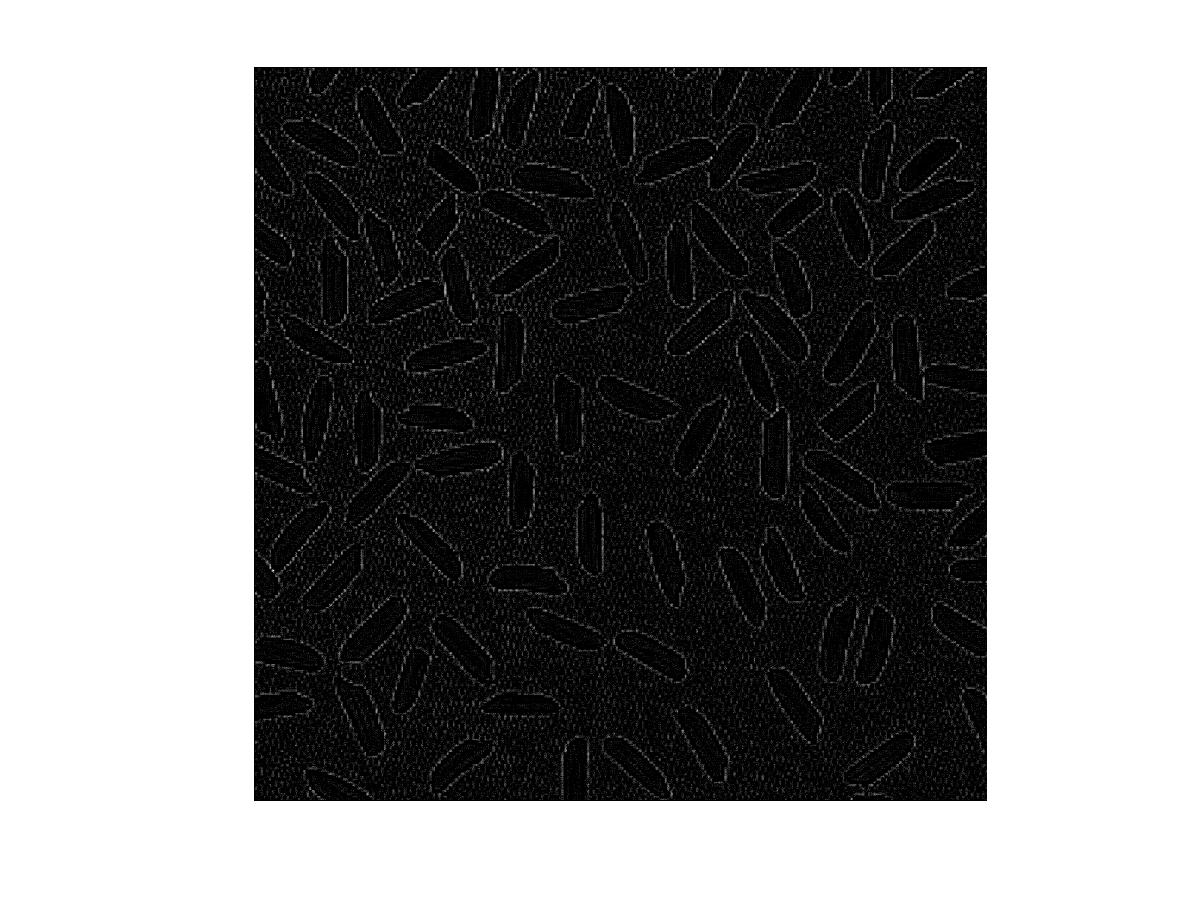
\includegraphics[width=0.8\textwidth]{Bordas.jpg}
        \caption{Image with edge filter.}
        \label{Bordas1}
    \end{figure}
\end{frame}

\end{document}
